\documentclass{article} % For LaTeX2e
\usepackage{nips15submit_e,times}
\usepackage{hyperref}
\usepackage{graphicx}
\usepackage{url}
%\documentstyle[nips14submit_09,times,art10]{article} % For LaTeX 2.09
\newcommand\BibTeX{B{\sc ib}\TeX}

\title{LSTM for Sentiment Analysis on Twitter}

\author{
Trapit Bansal
\And
Kate Silverstein
\And
Jun Wang
}

%% \author{
%% David S.~Hippocampus\thanks{ Use footnote for providing further information
%% about author (webpage, alternative address)---\emph{not} for acknowledging
%% funding agencies.} \\
%% Department of Computer Science\\
%% Cranberry-Lemon University\\
%% Pittsburgh, PA 15213 \\
%% \texttt{hippo@cs.cranberry-lemon.edu} \\
%% \And
%% Coauthor \\
%% Affiliation \\
%% Address \\
%% \texttt{email} \\
%% \AND
%% Coauthor \\
%% Affiliation \\
%% Address \\
%% \texttt{email} \\
%% \And
%% Coauthor \\
%% Affiliation \\
%% Address \\
%% \texttt{email} \\
%% \And
%% Coauthor \\
%% Affiliation \\
%% Address \\
%% \texttt{email} \\
%% (if needed)\\
%% }


% The \author macro works with any number of authors. There are two commands
% used to separate the names and addresses of multiple authors: \And and \AND.
%
% Using \And between authors leaves it to \LaTeX{} to determine where to break
% the lines. Using \AND forces a linebreak at that point. So, if \LaTeX{}
% puts 3 of 4 authors names on the first line, and the last on the second
% line, try using \AND instead of \And before the third author name.

\newcommand{\fix}{\marginpar{FIX}}
\newcommand{\new}{\marginpar{NEW}}

\nipsfinalcopy % Uncomment for camera-ready version

\begin{document}


\maketitle

\begin{abstract}
abstract goes here
\end{abstract}

\section{Introduction}

We use LSTM \cite{hochreiter1997long} to do stuff

\section{Related Work}

Dynamic convolutional neural net for sentences \cite{kalchbrenner2014convolutional}


sentiment specific word embeddings \cite{tang2014learning}


character-lvl CNN for text classification \cite{zhang2015character}

\section{Model}

\section{Results}

\subsection{Datasets}
We conduct our experiments on two datasets: the latest benchmark dataset for SemEval 2016 and the dataset provided by \cite{go2009twitter}. In the latter dataset, the training set consists of $1.6$ million weakly-supervised tweets collected during $2009$, and the test set is hand-labeled. In the experiments presented below, we first train our models on the Go dataset, then re-train the model parameters on the smaller, fully-supervised SemEval dataset.

\begin{table}[h!]
\centering
\caption{Data size and label distribution}
\label{my-label}
\begin{tabular}{|lllll|}
\hline
      & \multicolumn{2}{l}{Go et. al. (1.6M)} & \multicolumn{2}{l}{SemEval2016} \\
      & neg               & pos               & neg            & pos            \\
\hline
train & 800000            & 800000            & 781            & 2805           \\
dev   & -                 & -                 & 358            & 766            \\
test  & 177               & 182               & 286            & 886           \\
\hline
\end{tabular}
\end{table}

\subsection{Experiments}
We compare the performance of character-level models against word-level models. For the former, we compare across character sets (``utf8'' and ``ascii''), parameter initializations (``rnd'' and ``eye''), and embedding dimension sizes ($50$ and $200$). The vocabulary for the ``utf8'' setting consisted of $1949$ characters, and for ``ascii'' consisted of $93$ characters. We initialize model parameters randomly at all levels in the ``rnd'' setting whereas in the ``eye'' setting, we initialize the second-level LSTM cell and gate parameters using the identity matrix.

We compare word-level models under two settings: initializing the word embeddings using random vectors (``word/rnd'') and initialization using the embeddings provided in \cite{tang2014learning} (``word/sswe'').

We train all models using the implementation of the Adam algorithm \cite{kigma2014adam} provided in Lasagne \cite{lasagne} and a learning rate set to $0.1$ \footnote{We retrained the ascii/rnd/200 on SemEval using AdaGrad and a learning rate of $0.01$ to achieve $84.13$; using Adam and $0.1$ learning rate, the result was $83.21$}. 

\begin{table}[h!]
\centering
\caption{Accuracy across LSTMs}
\label{char-models}
\begin{tabular}{|l|ll|}
\hline
              & 1.6M (acc)          & semeval (acc) \\
\hline
ascii/rnd/50  & \textbf{83.84} & 82.08   \\
ascii/rnd/200 & 82.45          & \textbf{84.13}   \\
ascii/eye/50  & 77.44          & 79.18   \\
utf8          & 81.34          & 82.34   \\
word/rnd      & 81.85          & 78.07   \\
word/sswe     & 83.24          & 79.27   \\
\hline
\end{tabular}
\end{table}

The character-level models using the ``ascii'' character set outperformed the other models. It is worth noting that the ``utf8'' model performaed comparably despite having a much larger vocabulary size. It is not suprising that the ``utf8'' model performed worse than the ``ascii'' model, as the test data consisted of only English tweets; however, since the ``utf8'' model is implicitly multi-lingual, our results suggest that the same model may perform well across multiple languages. We leave such experiments for future work.

\subsection{Analysis}
Figure ~\ref{fig:cool} shows the effect of character repetition on model confidence over the course of the sequence, where confidence is computed using the softmax function:

$$P(y = j|\mathbf{x}) = \frac{e^{\mathbf{x}^T \mathbf{w}_j}}{\sum_{k=1}^{K} e^{\mathbf{x}^T \mathbf{w}_k}}$$

In our experiments, we had $K = 2$ corresponding to binary classification between ``positive'' and ``negative'' tweets. Sequences ending in periods (``cool.'', ``coool.'') ended up with less-confident scores than tweets not ending in periods. Repeated exclamation points don't increase the model's confidence in the ``positive'' label as much as might be expected. 

\begin{figure}[h!]
\label{fig:cool}
\begin{center}
%\framebox[4.0in]{$\;$}
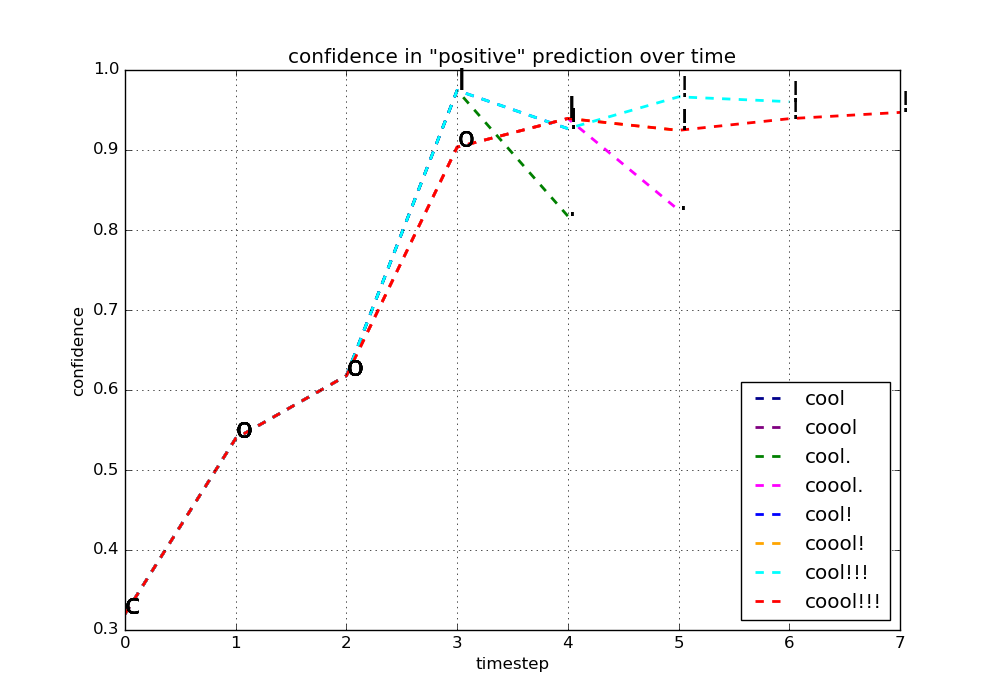
\includegraphics[width=0.95\textwidth]{figs/cool}
%\fbox{\rule[-.5cm]{0cm}{4cm} \rule[-.5cm]{4cm}{0cm}}
\end{center}
\caption{Sample figure caption.}
\end{figure}

Figure ~\ref{fig:puppies} shows that the character-level model learns word meaning at a lexical level: the predictions for ``I love puppies'' and ``I hate puppies'' diverges sharply after the model has finished reading ``lov'' (``love'') and ``hat'' (``hate'').

\begin{figure}[h!]
\label{fig:puppies}
\begin{center}
%\framebox[4.0in]{$\;$}
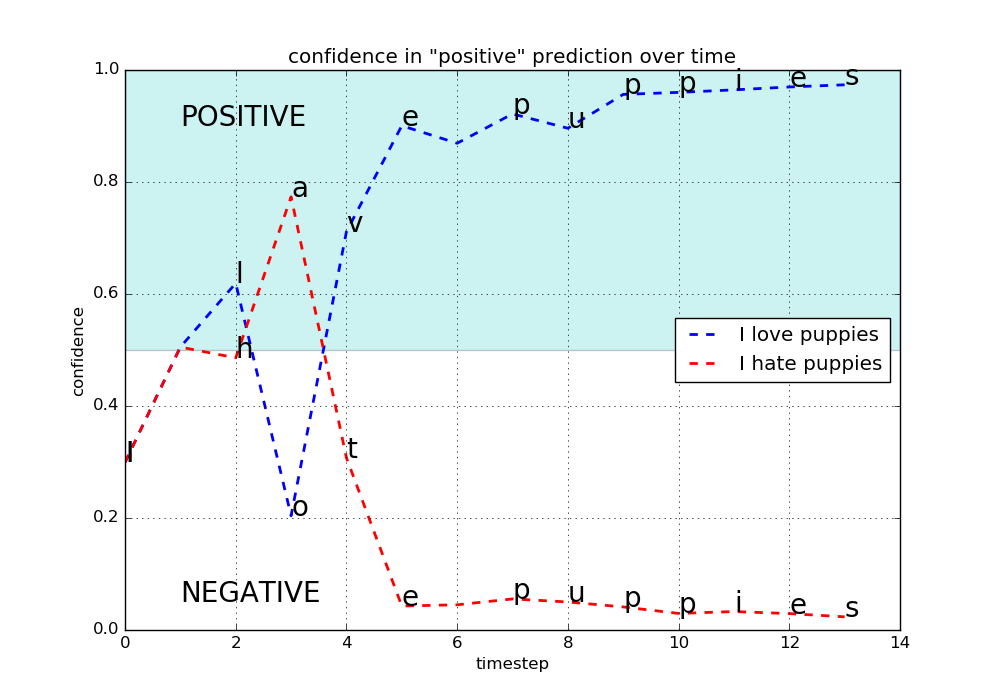
\includegraphics[width=0.95\textwidth]{figs/puppies}
%\fbox{\rule[-.5cm]{0cm}{4cm} \rule[-.5cm]{4cm}{0cm}}
\end{center}
\caption{Sample figure caption.}
\end{figure}

Figure ~\ref{fig:dentist} provides further evidence that character-level models can reason about lexical semantics in an intuitive fashion. We compare confidence contours across four tweets from the Go test set. The ground truth labels for the first two tweets are both ``negative'', and for the second two are both ``positive''. In the first two, the model finds strong evidence for a ``negative'' prediction before reaching the word ``dentist'', and correctly predicts that both tweets are ``negative''. In the second two, the word ``dentist'' results in an increase in the model's confidence in a ``negative'' prediction; however, the words ``enjoyable'' and ``:)'' cause the model's confidence to decrease in the ``positive'' direction. 

\begin{figure}[h!]
\label{fig:dentist}
\begin{center}
%\framebox[4.0in]{$\;$}
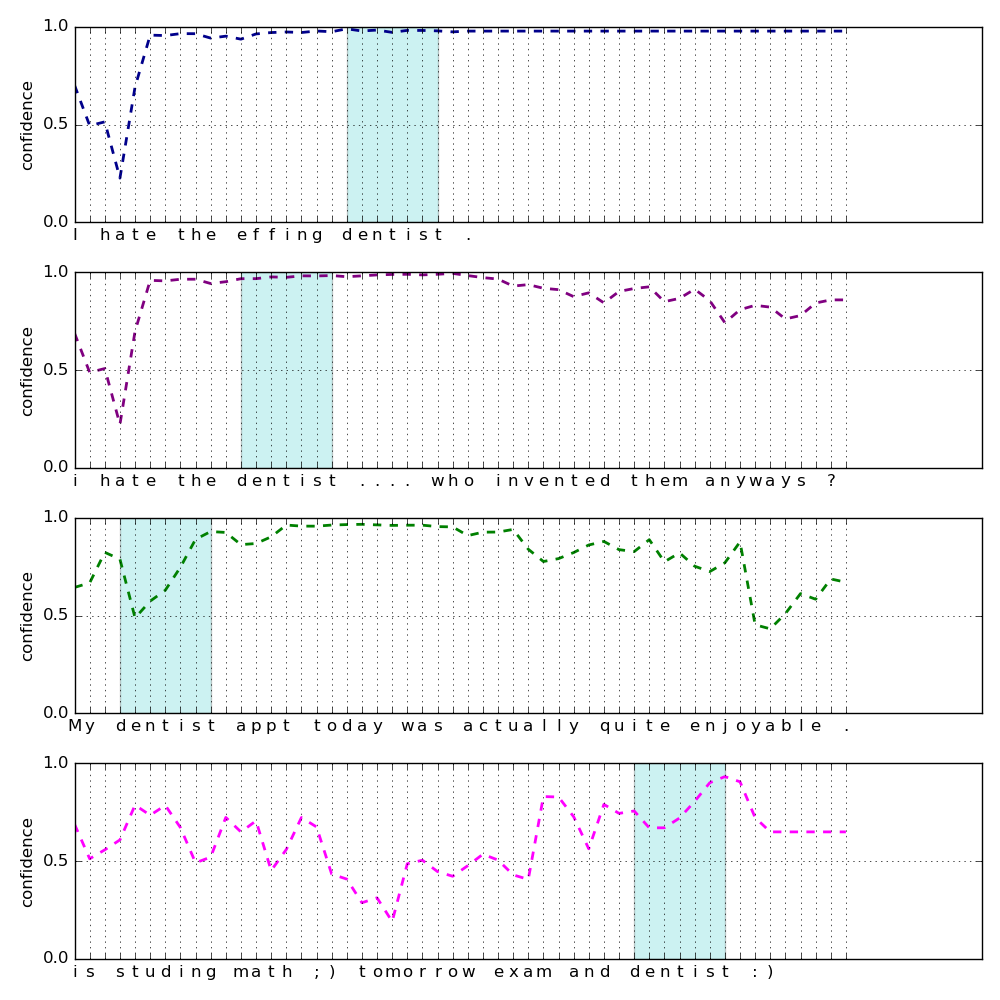
\includegraphics[width=0.95\textwidth]{figs/dentist}
%\fbox{\rule[-.5cm]{0cm}{4cm} \rule[-.5cm]{4cm}{0cm}}
\end{center}
\caption{Confidence in ``negative'' prediction over time}
\end{figure}

\section{Conclusion}


\subsubsection*{Acknowledgments}



\subsubsection*{References}

\bibliography{paper}
\bibliographystyle{plain}
%% References follow the acknowledgments. Use unnumbered third level heading for
%% the references. Any choice of citation style is acceptable as long as you are
%% consistent. It is permissible to reduce the font size to `small' (9-point) 
%% when listing the references. {\bf Remember that this year you can use
%% a ninth page as long as it contains \emph{only} cited references.}

%% \small{
%% [1] Alexander, J.A. \& Mozer, M.C. (1995) Template-based algorithms
%% for connectionist rule extraction. In G. Tesauro, D. S. Touretzky
%% and T.K. Leen (eds.), {\it Advances in Neural Information Processing
%% Systems 7}, pp. 609-616. Cambridge, MA: MIT Press.

%% [2] Bower, J.M. \& Beeman, D. (1995) {\it The Book of GENESIS: Exploring
%% Realistic Neural Models with the GEneral NEural SImulation System.}
%% New York: TELOS/Springer-Verlag.

%% [3] Hasselmo, M.E., Schnell, E. \& Barkai, E. (1995) Dynamics of learning
%% and recall at excitatory recurrent synapses and cholinergic modulation
%% in rat hippocampal region CA3. {\it Journal of Neuroscience}
%% {\bf 15}(7):5249-5262.
%% }

\end{document}
